\noindent Racial achievement gap is deeply ingrained in the United States. Before the Brown vs. Board of Education decision in 1954, school segregation by race was supported by laws throughout the South, where the great majority of blacks lived or from where they had recently emigrated. Although the achievement gap has declined significantly over the past 40 years, it remains quite large (see Figure 1) and failed to close further (Magnuson and Waldfogel, 2008). 
 
\begin{figure}[H]
  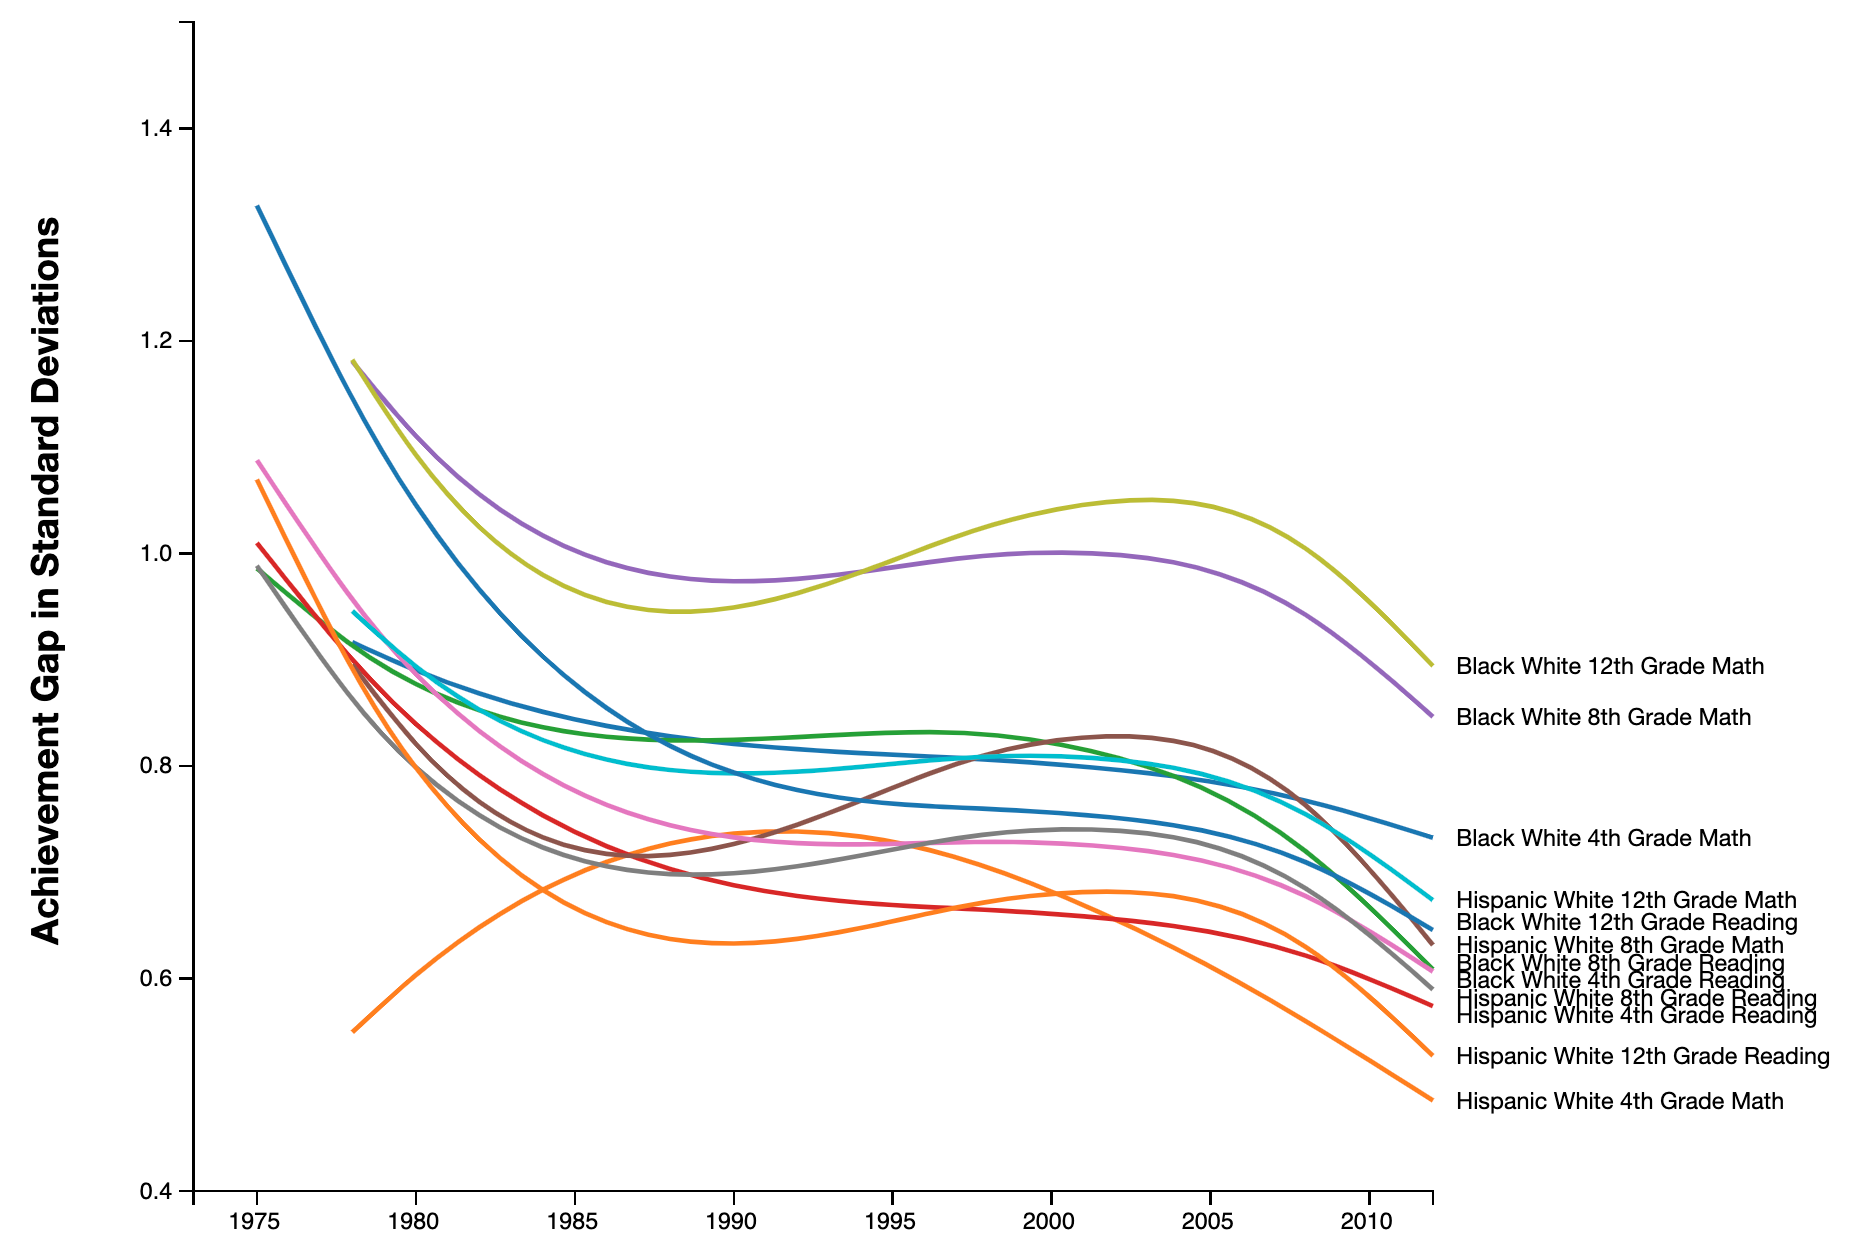
\includegraphics[width=\linewidth]{f1.png}
  \caption{The achievement gap, while narrowing significantly, remains quite large}
  \source{The Educational Opportunity Project, Stanford University}
  \label{fig:boat1}
\end{figure}

\noindent The Educational Opportunity Monitoring Project at Stanford University tracked the white-black achievement gap since 1970. The Project assesses performance using the National Assessment of Educational Progress (NAEP) math and reading tests of 9-, 13-, and 17-year-olds from around the United States. As Figure 1 shows, white-black achievement gaps have narrowed substantially since the 1970s, in all grades, and in both math and reading. As of the most recent data, the gaps were 30-40 percent smaller than they were in the 1970s. Regardless, very large differences between black and white students remain, ranging from 0.6 to 0.9 standard deviations, especially in math performance. Therefore, it is worth examining novel approaches proposed to close the achievement gap.

My research look at closing the achievement gap using culturally relevant pedagogy (CRP) that has been proposed by Ladson-Billings (1995) but haven't received public's attention until recently. I will contribute to a larger empirical literature on how effective CRP is on closing the racial achievement gap. I will first examine how implementation of the program is related with math percentage of proficiency; then I will focus on finding out which school level will generate the greatest effect, if any. 

\noindent Figure 2 provides a clearer idea of how serious the issue is in school districts in the US. The Stanford researchers also provide a more intuitive measure of achievement gap. They use school district level data to compare the academic performance of black and white 3-8 graders across the US. As recently as 2016, they find the difference in standardized test scores rises, by the time students are in the 8th grade, to approximately two years of schooling.

In the figure below, each circle represents a school district, with the size of the circle proportional to the number of students enrolled in that district. The black linear line crossing the origin indicates “no white/black disparity in test scores.” Circles below the line are districts where black students perform worse than white students; circles above the line represents the opposite. The farther a district sits away from the diagonal line, the greater the gap. 
 
\begin{figure}[H]
  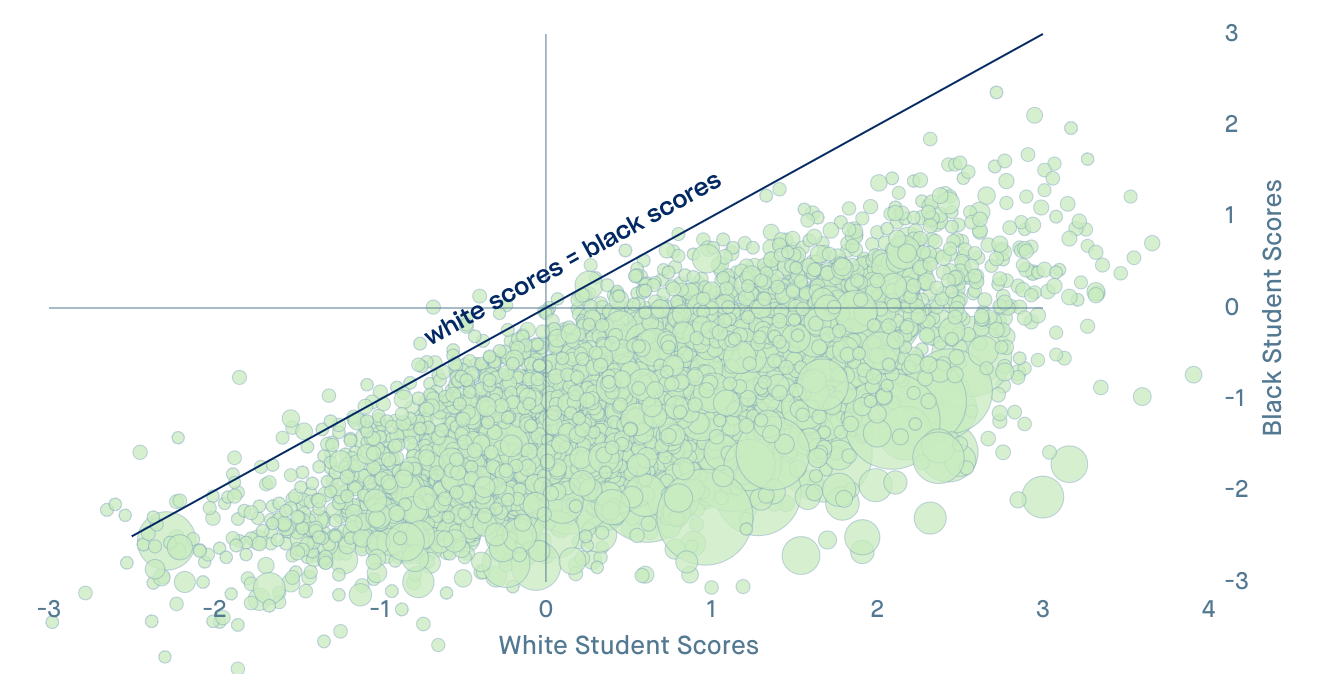
\includegraphics[width=\linewidth]{f2.png}
  \caption{In most school districts, black students in 2016 perform worse than white students}
  \source{The Educational Opportunity Project, Stanford University}
  \label{fig:boat1}
\end{figure}

This figure clearly shows that black students under-perform in the great majority of school districts. The achievement gap is systemic, not individual. Even decades after the end of legal segregation, a large and persistent achievement gap remains. 

